%
% 3-eulerlagrange.tex
%
% (c) 2023 Prof Dr Andreas Müller
%
\section{Die Euler-Lagrange Differentialgleichung
\label{buch:variation:section:eulerlagrange}}
\kopfrechts{Die Euler-Lagrange Differentialgleichung}
Das Neuartige an der Aufgabenstellung des Brachistochronenproblems
war, dass eine Funktion gesucht war, so dass ein damit gebildetes
Integral eine Minimaleigenschaft erfüllt.
Für die damalige Mathematik war die Aufgabe, eine Funktion zu finden,
nicht neu.
Die Theorie der Differentialgleichungen war bereits entwickelt,
Newton hat die Infinitesimalrechnung ja erfunden, um damit die
Bewegungsgleichungen der Physik zu formulieren und zu lösen.
In einer Differentialgleichung werden Werte und Ableitungen einer
Funktion an einer einzigen Stelle miteinander verbunden.
Etwas salop formuliert sagt die Differentialgleichung in jedem
Punkt, in welche Richtung und mit welcher Krümmung die Funktionskurve
weiter zu zeichnen ist.

Im Brachistochronenproblem tragen aber alle Werte der gesuchten
Funktion zum Integral bei, es scheint daher auf den ersten Blick
nicht möglich, das Problem durch schrittweise Konstruktion
``von Punkt zu Punkt'' der Lösungskurve zu konstruieren.

Bernoullis Lösung des Brachistochrononproblems beruht auf der
Beobachtung, dass sich die Bedingung für die schnellste Bahn
durch eine Bedingung ersetzen lässt, die in jedem einzelnen
Punkt ausgewertet werden kann.
Das von ihm verwendete Fermat-Prinzip wurde ursprünglich ebenfalls
als eine globale Eigenschaft eines Lichtstrahls formuliert.
Aus dem Fermat-Prinzip folgt aber das Brechungsgesetz, welches
sagt, dass die Richtung eines Strahls in einem Punkt genau dann
ändert, wenn sich dort auch der Brechungsindex der beiden Medien
ändert.
Das Fermat-Prinzip ist also ein Beispiel dafür, wie eine globale
Bedingung erfüllt werden kann, indem einer lokalen Regel in jedem
Punkt gefolgt wird.

Es ist das Verdienst von Euler und Lagrange, zu erkennen, dass diese
Übersetzung eines globalen Variationsproblems in ein lokales 
Problem immer möglich ist.
Es entsteht dabei die Euler-Lagrange-Differentialgleichung, welche
die Problemstellung auf die Lösung einer Differentialgleichung
reduziert.
Damit ist ein allgemein anwendbares Lösungsverfahren gefunden.
Zu einem Variationsproblem lässt sich immer eine Differentialgleichung
finden, welche die gesuchte Funktion als Lösung hat.

In diesem Abschnitt soll dieser indirekte Weg der Lösung von
Variationsaufgaben dargestellt werden.
Wir werden später zeigen, dass diese Vorgehensweise nicht immer
erfolgreich sein kann.
Zum Beispiel werden wir in Kapitel~\ref{buch:chapter:nichtdiff}
Variationsprobleme kennenlernen, deren Lösungskurven nicht
differenzierbar sind und daher auch nicht von einer Differentialgleichung
gefunden werden können.
Im Kapitel~\ref{buch:chapter:direkt} werden daher die sogenannten
direkten Methodn vorgestellt, die den Umweg über eine
Differentialgleichung vermeiden.

%
% 31-lagrangefunktion.tex
%
% (c) 2023 Prof Dr Andreas Müller
%

%
% Die Lagrange-Funktion
%
\subsection{Die Lagrange-Funktion
\label{buch:variation:eulerlagrange:subsection:lagrange-funktion}}
Wir betrachten Variationsprobleme der folgenden Art.
Gesucht ist eine auf dem Intervall $[x_0,x_1]$ definirte
Funktion $y(x)$, die das Integral
\begin{equation}
I(y)
=
\int_{x_0}^{x_1}
F(x, y(x), y'(x))
\,dx
\label{buch:variation:eulerlagrange:eqn:funktional}
\end{equation}
maximiert oder minimiert.
Der Ausdruck~\eqref{buch:variation:eulerlagrange:eqn:funktional}
wird ein Funktional genannt.
Die Funktion
\[
F
\colon
\mathbb{R}\times
\mathbb{R}\times
\mathbb{R}
\to
\mathbb{R}
\]
von drei Variablen heisst die {\em Lagrange-Funktion}
des Funktionals \eqref{buch:variation:eulerlagrange:eqn:funktional}.

\begin{beispiel}
Die Lagrange-Funktion des Brachistochronenproblems ist
\[
F(x,y,y')
=
\sqrt{ \frac{1+y^{\prime 2}}{y} }.
\]
Die Funktion hängt nicht von $x$ ab, was bedeutet, dass eine
Verschiebung in $x$-Richtung die Form der Lösungsfunktion des
Variationsproblems nicht ändert.
\end{beispiel}

\begin{beispiel}
\label{buch:variation:eulerlagrange:beispiel:gerade}
Wir formulieren die Aufgabe, die kürzeste Verbindung der Punkte
$(x_0,y_0)$ und $(x_1,y_1)$ in einer Ebene zu finden, als Variationsproblem.
Die Länge einer Kurve $y(x)$ ist das Integral
\[
l(y)
=
\int_{x_0}^{x_1}
\sqrt{1+y'(x)^2}\,dx.
\]
Daraus lesen wir ab, dass die Lagrange-Funktion dieses Variationsproblems
\begin{equation}
F(x,y,y') = \sqrt{1+y^{\prime 2}}
\label{buch:variation:eulerlagrange:eqn:geradeL}
\end{equation}
ist.
Die Funktion hängt weder von $x$ noch von $y$ ab.
Dies ist auch zu erwarten, denn die Länge einer Kurve hängt nicht davon
ob, wo in der Ebene sie platziert ist.
Eine Verschiebung in $x$-Richtung würde das $x$-Argument ändern,
eine Verschiebung in $y$-Richtung die $y$-Werte.
Wäre $F$ von $x$ oder $y$ abhängig, könnte auch die Länge der Kurve
davon abhängen.
\end{beispiel}


%
% 32-eulerlagrangedgl.tex
%
% (c) 2023 Prof Dr Andreas Müller
%

%
% Euler-Lagrange_Differentialgleichung
%
\subsection{Euler-Lagrange-Differentialgleichung
\label{buch:variation:eulerlagrange:subsection:dgl}}
%
% variation0.tex -- Variation mit festen Enden
%
% (c) 2021 Prof Dr Andreas Müller, OST Ostschweizer Fachhochschule
%
\documentclass[tikz]{standalone}
\usepackage{amsmath}
\usepackage{times}
\usepackage{txfonts}
\usepackage{pgfplots}
\usepackage{csvsimple}
\usetikzlibrary{arrows,intersections,math}
\definecolor{darkred}{rgb}{0.8,0,0}
\begin{document}
\def\skala{1}
\def\xzero{1}
\def\xone{10}
\def\yzero{1}
\def\yone{5}
\begin{tikzpicture}[>=latex,thick,scale=\skala,
declare function={
	x(\t)   = (1-\t)*\xzero+\t*\xone;
	t(\x)   = (\x-\xzero)/(\xone-\xzero);
	eta(\t) = \t*(1-\t)*(2*cos(180*\t)+4*\t*sin(720*\t)+6);
	y(\t)   = (1-\t)*\yzero+\t*\yone+4*\t*(1-\t);
}]

\draw (\xzero,-0.05) -- (\xzero,0.05);
\draw (-0.05,\yzero) -- (0.05,\yzero);
\draw[line width=0.2pt] (\xzero,0) -- (\xzero,\yzero);
\draw[line width=0.2pt] (0,\yzero) -- (\xzero,\yzero);
\node at (\xzero,-0.05) [below] {$x_1\mathstrut$};
\node at (-0.05,\yzero) [left] {$y_1\mathstrut$};

\draw (\xone,-0.05) -- (\xone,0.05);
\draw (-0.05,\yone) -- (0.05,\yone);
\draw[line width=0.2pt] (\xone,0) -- (\xone,\yone);
\draw[line width=0.2pt] (0,\yone) -- (\xone,\yone);
\node at (\xone,-0.05) [below] {$x_2\mathstrut$};
\node at (-0.05,\yone) [left] {$y_2\mathstrut$};

\fill[color=darkred] (\xzero,\yzero) circle[radius=0.08];
\fill[color=darkred] (\xone,\yone) circle[radius=0.08];
\node at (\xzero,\yzero) [above left] {$P_1$};
\node at (\xone,\yone) [right] {$P_2$};

\foreach \e in {-1.6,-1.2,...,1.7}{
	\draw[color=gray,smooth] plot[domain=0:1] ({x(\x)},{y(\x)+\e*eta(\x)});
}
\node[color=gray] at (3.6,5.65) {$y(x)+\varepsilon\eta(x)$};

\draw[color=darkred,smooth,line width=1.4pt] plot[domain=0:1] ({x(\x)},{y(\x)});
\node[color=darkred] at (6.8,4.8) {$y(x)$};

\draw[->] (-0.1,0) -- (11.6,0) coordinate[label={$x$}];
\draw[->] (0,-0.1) -- (0,8) coordinate[label={right:$y$}];

\end{tikzpicture}
\end{document}


Das Maximum oder Minimum einer Funktionen mehrere Variablen wurde
gefunden, indem die Richtungsableitung berechnet und $=0$ gesetzt
wurde.
Um die Funktion zu bestimmen, die ein Funktional $I(y)$ zu einem
Maximum oder Minimum macht, versuchen wir, die Idee der Richtungsableitung
für ein Funktional nachzuahmen.
Wir nehmen daher an, dass $y(x)$ eine Funktion ist, die das Funktional
$I(y)$ zu einem Minimum macht.
Für die Richtungsableitung addieren wir ein Vielfaches einer
Funktion $\eta(x)$, die Summe $y(x)+\varepsilon\eta(x)$ entspricht
dann einer Geraden mit Richtung $\eta(x)$ im Funktionenraum
(Abbildung~\ref{buch:variation:fig:variation0}).
Die Funktionen $y(x)+\varepsilon\eta(x)$ sind aber nur dann Kandidaten
für eine Lösung des Problems, wenn immer noch
\begin{align*}
y(x_0) + \varepsilon \eta(x_0) &= y_0
&&\text{und}&
y(x_1) + \varepsilon \eta(x_1) &= y_1
\end{align*}
gilt.
Dies ist nur möglich, wenn $\eta(x_0)=\eta(x_1)=0$ ist.

Wir berechnen jetzt die Ableitung der Funktion
$\varepsilon\mapsto I(y+\varepsilon\eta )$ an der Stelle $\varepsilon=0$.
Da die Intervallgrenzen nicht von $\varepsilon$ abhängen, können wir
die Ableitung unter das Integral nehmen:
\begin{align*}
\frac{d}{d\varepsilon}
I(y+\varepsilon\eta)
&=
\int_{x_0}^{x_1}
\frac{d}{d\varepsilon}
F(x,y(x)+\varepsilon\eta(x),y(x)+\varepsilon\eta'(x))
\,dx.
\intertext{Da $F$ differenzierbar ist, kann die Ableitung mit der
Kettenregel berechnet werden, sie ist}
&=
\int_{x_0}^{x_1}
\frac{\partial F}{\partial y}
(x,y(x)+\varepsilon\eta(x),y(x)+\varepsilon\eta'(x))
\eta(x)
\\
&\qquad
+
\frac{\partial F}{\partial y'}
(x,y(x)+\varepsilon\eta(x),y(x)+\varepsilon\eta'(x))
\eta'(x)
\,dx.
\intertext{Uns interessiert aber nur der Wert an der Stelle $\varepsilon=0$,
er ist}
\frac{d}{d\varepsilon}
I(y+\varepsilon\eta)
\bigg|_{\varepsilon=0}
&=
\int_{x_0}^{x_1}
\frac{\partial F}{\partial y}
(x,y(x),y'(x))
\,
\eta(x)
+
\frac{\partial F}{\partial y'}
(x,y(x),y'(x))
\,
\eta'(x)
\,dx
=0.
\end{align*}
Das Integral hängt von den verschiedenen Faktoren $\eta(x)$ und
von $\eta'(x)$ in den beiden Termen unter dem Integral ab.
Wir integrieren den zweiten Term partiell 
\begin{align*}
\int_{x_0}^{x_1}
\frac{\partial F}{\partial y'}(x,y(x),y'(x))\,\eta'(x)\,dx
&=
\biggl[
\frac{\partial F}{\partial y'}(x,y(x),y'(x))\,\eta(x)
\biggr]_{x_0}^{x_1}
\\
&\qquad
-
\int_{x_0}^{x_1}
\frac{d}{dx}
\frac{\partial F}{\partial y'}(x,y(x),y'(x))\,\eta(x)\,dx.
\end{align*}
Da $\eta(x_0)=\eta(x_1)=0$ verschwindet der erste Term
auf der rechten Seite, es bleibt
\[
\frac{d}{d\varepsilon}
I(y+\varepsilon\eta)
\bigg|_{\varepsilon=0}
=
\int_{x_0}^{x_1}
\biggl(
\frac{\partial F}{\partial y}
(x,y(x),y'(x))
-
\frac{d}{dx}
\frac{\partial F}{\partial y'}
(x,y(x),y'(x))
\biggr)
\eta(x)
\,dx.
\]
Dies kann auch als Skalarprodukt
\[
\biggl\langle 
\frac{\partial F}{\partial y}
(x,y(x),y'(x))
-
\frac{d}{dx}
\frac{\partial F}{\partial y'}
(x,y(x),y'(x))
,
\eta(x)
\biggr\rangle
=
0
\]
geschrieben werden.
Da dies für jede differenzierbare Funktion $\eta$ mit Randwerten
$\eta(x_0)=\eta(x_1)$ gelten muss, folgt nach dem
Fundamentallemma~\ref{buch:variation:fundamentallemma:satz:fundamentallemma},
der folgende Satz. 

\begin{satz}[Euler-Lagrange]
\label{buch:variation:eulerlagrange:satz:eulerlagrange}
Wenn die mindestens zweimal stetig differenzierbare Funktion $y(x)$
unter allen solchen Funktionen mit $y(x_0)=y_0$ und $y(x_1)=y_1$
das Funktional
\[
I(y)
=
\int_{x_0}^{x_1}
F(x,y(x),y'(x))\,dx
\]
zu einem Maximum oder Minimum macht, dann ist $y(x)$ eine Lösung der
gewöhnlichen Differentialgleichung
\begin{equation}
\frac{d}{dx}
\frac{\partial F}{\partial y'}(x,y(x),y'(x))
-
\frac{\partial F}{\partial y}(x,y(x),y'(x))
=
0.
\label{buch:variation:eulerlagrange:eqn:eulerlagrange}
\end{equation}
Sie heisst die {\em Euler-Lagrange-Differentialgleichung}.
\end{satz}

Eine Lösung des Variationsproblems kann also als Lösung der
Euler-Lagrange-Dif\-fe\-ren\-tial\-glei\-chung mit den Randwerten
$y(x_0)=x_0$ und $y(x_1)=y_1$ gefunden werden.
Die Bedingung ist notwendig, aber nicht hinreichend.
Wie bei der Bestimmung eines Extremums bei Funktionen endlich
vieler Variablen garantiert das Verschwinden der Richtungsableitung
nicht, dass auch tatsächlich ein Extremum vorliegt.
Man sagt daher auch, dass eine Lösung $y(x)$ der
Euler-Lagrange-Differentialgleichung das Funktional $I(y)$
stationär macht.

Eine weitere Einschränkung ist, dass die Herleitung der
Euler-Lagrange-Differential\-gleichung vorausgesetzt hat,
dass die Lösungsfunktion $y(x)$ mindestens zweimal 
stetig differenzierbar ist.
Es gibt aber durchaus Variationsprobleme, deren Lösungen
nicht differenzierbar sind, dazu mehr im Kapitel~\ref{buch:chapter:nichtdiff}.

\begin{beispiel}
\label{buch:variation:eulerlagrange:beispiel:gerade}
Wir lösen das Variationsproblem von Beispiel
\ref{buch:variation:eulerlagrange:beispiel:gerade}
mit der Lagrange-Funk\-tion
\eqref{buch:variation:eulerlagrange:eqn:geradeL}.
Da die Lagrange-Funktion nicht von $y$ abhängt, bleibt von der 
Euler-Lagrange-Gleichung nur
\[
\frac{d}{dx}
\frac{\partial L}{\partial y'}(x,y(x),y'(x))
=
0
\]
übrig.
Berechnung der Ableitung liefert
\begin{equation}
\frac{\partial}{\partial y'}
\sqrt{1+y^{\prime 2}}
=
\frac{y'}{\sqrt{1+y^{\prime 2}}}.
\label{buch:variation:eulerlagrange:eqn:ableitungFyp}
\end{equation}
Die Ableitung nach $x$ ergibt
\begin{align*}
\frac{d}{dx}
\frac{\partial}{\partial y'}
\sqrt{1+y^{\prime 2}}
&=
\frac{d}{dx}
\frac{y'}{\sqrt{1+y^{\prime 2}}}
\\
&=
\frac{
y''\sqrt{1+y^{\prime 2}}-y'\cdot \frac{y'y''}{\sqrt{1+y^{\prime 2}}}
}{
1+y^{\prime 2}
}
\\
&=
y''
\frac{
1+y^{\prime 2}-y^{\prime 2}
}{
(1+y^{\prime 2})^{\frac32}
}.
\intertext{Die Euler-Lagrange-Differentialgleichung ist daher}
0
&=
\frac{y''}{(1+y^{\prime 2})^{\frac32}} .
\end{align*}
Der Nenner auf der rechten Seite ist immer $\ge 1$, die Gleichung kann
also nur erfüllt sein, wenn $y''=0$ ist.
Die Funktion $y(x)$ muss also eine lineare Funktion $y=ax+b$ sein.
Die Randbedingung wird erfüllt für die Geradengleichung
\[
y(x)
=
\frac{y_1-y_0}{x_1-x_0}(x-x_0) + y_0.
\]
Kürzeste Verbindungen in der Ebene sind daher Geraden.
\end{beispiel}


%
% 33-brachistochrone.tex
%
% (c) 2023 Prof Dr Andreas Müller
%

%
% Lösung des Brachistochronenproblems
%
\subsection{Lösung des Brachistochronenproblems
\label{buch:variation:eulerlagrange:subsection:brachistochrone}}
Das Brachistochronenproblem kann jetzt mit Hilfe der
Euler-Lagrange-Differential\-glei\-chung gelöst werden.
Dazu muss zunächst die Lagrange-Funktion ermittelt werden,
mit der dann die Euler-Lagrange-Differentialgleichung aufgestellt
werden kann.
Dies erfordert einiges an Rechnung.
Schliesslich muss die Differentialgleichung gelöst werden.

%
% Lagrange-Funktion
%
\subsubsection{Lagrange-Funktion}
Die Lagrange-Funktion für das Brachistochronenproblem ist
\[
L(x,y,y')
=
\sqrt{\frac{1+y^{\prime 2}}{y}}.
\]
Diese Form des Variationsprinzips unterscheidet sich von der früher
gefundenen nur durch einen konstanten Faktor, der keinen Einfluss
auf die Lösung hat.

%
% Partielle Ableitungen der Lagrange-Funktion
%
\subsubsection{Partielle Ableitungen der Lagrange-Funktion}
Für die Euler-Lagrange-Differentialgleichung werden die partiellen
Ableitungen nach $y$ und $y'$ benöigt, sie sind
\begin{align*}
\frac{\partial L}{\partial y}
&=
-
\frac{\!\sqrt{1+y^{\prime 2}}}{2y^{\frac32}}
&&\Rightarrow
&\frac{\partial L}{\partial y}\bigl(x,y(x),y'(x)\bigr)
&=
\frac{\!\sqrt{1+y'(x)^2}}{2y(x)^{\frac32}}
\\
\frac{\partial L}{\partial y'}
&=
\frac{y'}{\!\sqrt{y\cdot (1+y^{\prime 2})}}
&&\Rightarrow
&
\frac{\partial L}{\partial y'}\bigl(x,y(x),y'(x)\bigr)
&=
\frac{y'(x)}{\!\sqrt{y(x)(1+y'(x)^2)}},
\end{align*}
wobei wir auf der rechten Seite bereits die Funktionen $y(x)$ und $y'(x)$
eingesetzt haben.
Für die Euler-Lagrange-Differentialgleichung muss die $y'$-Ableitung
nach $x$ ableiten werden, dies ergibt
\begin{align*}
\frac{d}{dx}
\frac{\partial L}{\partial y'}\bigl(x,y(x),y'(x)\bigr)
&=
\frac{d}{dx}
\frac{y'(x)}{\!\sqrt{y(x)(1+y'(x)^2)}},
\\
&=
\frac{
y''(x)
\!\sqrt{y(x)(1+y'(x)^2)}
-
y'(x)
\displaystyle\frac{
		y'(x) (1+y'(x)^2) + 2y(x)y'(x)y''(x)
	}{
		2\sqrt{y(x)(1+y'(x)^2)}
}
}{
y(x)(1+y'(x)^2)
}
\\
&=
\frac{
2y''(x)
y(x)(1+y'(x)^2)
-
y'(x)
\bigl(y'(x)(1+y'(x)^2)+2y(x)y'(x)y''(x)\bigr)
}{
2\bigl(y(x)(1+y'(x)^2)\bigr)^{\frac32}
}
\\
&=
\frac{
2y(x)y''(x) + 2y(x)y'(x)^2y''(x)
-y'(x)^2-y'(x)^4-2y(x)y'(x)^2y''(x)
}{
2\bigl(y(x)(1+y'(x)^2)\bigr)^{\frac32}
}
\\
&=
\frac{
2y(x)y''(x) -y'(x)^2-y'(x)^4
}{
2\bigl(y(x)(1+y'(x)^2)\bigr)^{\frac32}
}.
\intertext{Um den anderen Term der Euler-Lagrange-Differentialgleichung
auf den gleichen Nenner zu bringen, muss mit $(1+y'(x)^2)^\frac32$
erweitert werden:
}
\frac{\partial L}{\partial y}\bigl(x,y(x),y'(x)\bigr)
&=
-
\frac{
(1+y'(x)^2)^2
}{
2\bigl(y(x)(1+y'(x)^2)\bigr)^{\frac32}
}
=
\frac{-1-2y'(x)^2-y'(x)^4}{
2\bigl(y(x)(1+y'(x)^2)\bigr)^{\frac32}
}
.
\end{align*}

%
% Euler-Lagrange-Differentialgleichung des Brachistochronenproblems
%
\subsubsection{Euler-Lagrange-Differentialgleichung des
Brachistochronenproblems}
Damit kann man jetzt die Euler-Lagrange-Differentialgleichung
\begin{align*}
0
&=
\frac{\partial L}{\partial y}\bigl(x,y(x),y'(x)\bigr)
-
\frac{d}{dx}
\frac{\partial L}{\partial y'}\bigl(x,y(x),y'(x)\bigr)
\\
&=
\frac{
-1 - 2y'(x)^2 - y'(x)^4
-2y(x)y''(x)+y'(x)^2+y'(x)^4
}{
2
\bigl(
y(x)
(1+y'(x)^2)
\bigr)^{\frac32}
}
\\
&=
\frac{
-1 - y'(x)^2
-2y(x)y''(x)
}{
2
\bigl(
y(x)
(1+y'(x)^2)
\bigr)^{\frac32}
}
\end{align*}
zusammenstellen.
Der Faktor $1+y'(x)^2$ im Nenner verschwindet nicht und die
Aufgabenstellung worde so parametrisiert, dass $y(x)>0$ ausser
im Startpunkt.
Die Gleichung ist daher nur erfüllt, wenn der Zähler
\begin{equation}
1+y'(x)^2+2y(x)y''(x)=0
\qquad\Rightarrow\qquad
y''(x)
=
-\frac{1+y'(x)^2}{2y(x)}
\label{buch:variation:eulerlagrange:eqn:brachistochrone0}
\end{equation}
ist.
Diese Differentialgleichung ist nicht ganz einfach zu lösen.

%
% Reduktion auf eine Differentialgleichung erster Ordnung
%
\subsubsection{Reduktion auf eine Differentialgleichung erster Ordnung}
Der folgende Trick hilft mit der Lösung der Differentialgleichung weiter.
Wir mutliplizieren die Gleichung
\eqref{buch:variation:eulerlagrange:eqn:brachistochrone0}
mit $y'(x)$ und erhalten
\begin{equation}
y'(x) + 2y(x)y'(x)y''(x) + y'(x)^3 = 0.
\label{buch:variation:eulerlagrange:eqn:multiplikation}
\end{equation}
Die ist die Ableitung
\begin{align*}
\bigl(
y(x)(1+y'(x)^2)
\bigr)'
&=
y'(x)(1+y'(x)^2)
+
y(x)(2y'(x)y''(x))
\\
&=
y'(x) + y'(x)^3
+2y(x)y'(x)y''(x).
\end{align*}
Die ursprüngliche Differentialgleichung wird damit zur Gleichung
\[
\bigl(
y(x)(1+y'(x)^2)
\bigr)'
=
0,
\]
die integriert werden kann und
\[
y(x)(1+y'(x)^2)
=
C
\]
für eine Integrationskonstante $C$, die aus den Randbedingungen
ermittelt werden muss, ergibt.
Diese Differentialgleichung kann in die explizite Form
\begin{equation}
y'(x)
=
\sqrt{
\frac{C-y(x)}{y(x)}
}
\label{buch:variation:eulerlagrange:eqn:brachistochrone1}
\end{equation}
gebracht werden.
Dies ist die gesuchte Differentialgleichung erster Ordnung.

%
% Lösung in Parameterdarstellung
%
\subsubsection{Lösung in Parameterdarstellung}
Aus der optischen Analogie von Bernoulli wissen wir, dass die Lösungskurve
möglicherweise besser durch den Winkel zwischen der Kurve und der Vertikalen
parametrisiert werden kann.
Wir bezeichnen den Winkel mit $\vartheta$ und schreiben die Ableitung
\[
\frac{dy}{dx}
=
\cot \vartheta
\qquad\Rightarrow\qquad
\tan \vartheta
=
\sqrt{\frac{y(\vartheta)}{C-y(\vartheta)}}
\qquad\Rightarrow\qquad
\frac{y(\vartheta)}{C-y(\vartheta)}
=
\frac{\sin^2 \vartheta}{\cos^2 \vartheta}.
\]
Ausmultiplizieren ergibt die Gleichung
\[
y(\vartheta)\cos^2\vartheta +y(\vartheta)\sin^2\vartheta) = y(\vartheta) = C\sin^2\vartheta.
\]
Die Ableitung nach $t$ ergibt
\[
\dot{y}
=
2C\sin \vartheta\cos \vartheta.
\]
Wegen
\[
y'(x)
=
\frac{\dot{y}}{\dot{x}}
=
\sqrt{ \frac{y}{C-y}}
\]
folgt
\[
\dot{x}(\vartheta)
=
\sqrt{\frac{y(\vartheta)}{C-y(\vartheta)}}
\cdot\dot{y}(\vartheta)
=
\frac{\sin \vartheta}{\cos \vartheta}\cdot 2 C\sin \vartheta\cos \vartheta
=
2C\sin^2\vartheta
=
C(1-\cos 2\vartheta).
\]
Durch Integrieren erhält man
\[
x(\vartheta)
= 
C\vartheta - \frac{C}{2}\sin 2\vartheta
+ x_0
=
\frac{C}2(2\vartheta-\sin 2\vartheta)+x_0
\]
mit der Integrationskonstanten $x_0$, die die Bedeutung der $x$-Koordinate
für einen Punkt hat, in dem die Kurve vertikal ist.
Da wir eine Lösung suchen, die im Punkt $(0,0)$ beginnt, muss $x_0=0$ sein.
Damit ist jetzt die Parameterdarstellung
\[
\begin{pmatrix}
x(\vartheta)\\
y(\vartheta)
\end{pmatrix}
=
\frac{C}{2}
\begin{pmatrix}
2t - \sin 2\vartheta\\
2\sin^2 \vartheta
\end{pmatrix}
=
\frac{C}{2}
\begin{pmatrix}
2\vartheta - \sin 2\vartheta\\
1  - \cos 2\vartheta
\end{pmatrix}.
\]
In allen Formeln kommt nur $2\vartheta$ vor, wir schreiben daher
$t=2\vartheta$ und erhalten die Paramterdarstellung
\begin{equation}
\begin{pmatrix}
y(t)\\
x(t)
\end{pmatrix}
=
\frac{C}{2}
\begin{pmatrix}
t-\sin t\\
1-\cos t
\end{pmatrix}
\label{buch:variation:eulerlagrange:eqn:zykloide}
\end{equation}
Diese Parametrisierung beschreibt eine Zykloide.
Sie beschreibt den Weg eines Punktes auf dem Umfang eines Kreises
vom Durchmesser $C$, der auf der $x$-Achse abgerollt wird.

%
% Randbedingungen
%
\subsubsection{Randbedingungen}
Die Konstanten $C$ muss so gewählt werden, dass die Lösungskurve
durch den Punkt $B=(x_B,y_B)$ geht. 
Sei $t_B$ der Wert des zugehörigen Parameters.
Wegen
\[
\frac{y_B}{x_B}
=
\frac{(C/2)(1-\cos t_B)}{(C/2)(t_B-\sin t_B)}
=
\frac{1-\cos t_B}{t_B-\sin t_B}
\]
muss $t$ eine Lösung der transzendenten Gleichung
\[
y_B(t_B-\sin t_B)=x_B(1-\cos t_B)
\]
sein, sie kann nur numerisch gelöst werden.
Sobald $t$ bestimmt ist, kann auch $C$ mit Hilfe von
\[
y_B = \frac{C}2(1-\cos t_B)
\qquad\Rightarrow\qquad
C
=
\frac{2y_B}{1-\cos t_B}
\]
eindeutig bestimmt werden.

%
% Singuläre Lösungen
%
\subsubsection{Singuläre Lösungen}
%
% bracchloes.tex
%
% (c) 2024 Prof Dr Andreas Müller
%
\begin{figure}
\centering
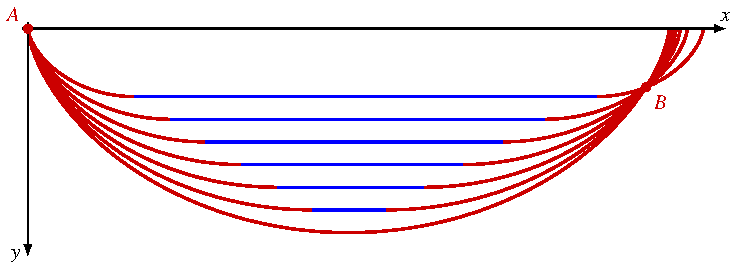
\includegraphics{chapters/020-variation/images/singulaer.pdf}
\caption{Verschiedene Lösungen unter Verwendung der singulären Lösungen
der Differentialgleichung der Brachistochronen.
Die roten Kurventeile sind Lösungen der ursprünglichen
Brachistochronengleichung
\eqref{XXX},
die blauen Teile sind durch die Multiplikation mit $y'$ in
\eqref{buch:variation:eulerlagrange:eqn:multiplikation}
hinzugekommen, sind aber nicht Lösungen der ursprünglichen
Gleichungen.
Nur die untereste Kurve ist daher eine Brachistochrone.
\label{buch:variation:eulerlagrange:fig:brachloes}}
\end{figure}

Die Differentialgleichung
\eqref{buch:variation:eulerlagrange:eqn:brachistochrone1}
hat die Lösung $y(x)=C$, denn in diesem Fall verschwindet
der Zähler und die Differentialgleichung wird zu $y'(x)=0$,
was für die Konstanten $C$ natürlich erfüllt ist.
Der Satz von Picard-Lindelöf besagt, dass die Lösung einer
Differentialgleichung $y'=f(x,y)$ eindeutig bestimmt ist, wenn die rechte
Seite eine Lipshitz-Bedingung erfüllt.
Dies ist für die rechte Seite von
\eqref{buch:variation:eulerlagrange:eqn:brachistochrone1}
nicht gegeben, die Lösung ist daher nicht eindeutig bestimmt.

Die Zykloide~\eqref{buch:variation:eulerlagrange:eqn:zykloide}
erreicht den tiefsten Punkt bei $t=\pi$, die $y$-Koordinate ist
$y(\pi)=C$.
In diesem Punkt ist die Lösungskurve horizontal.
Da die Lösung an diesem Punkt nicht eindeutig bestimmt ist,
kann sie mit der konstanten Funktion fortgesetzt werden
(Abbildung~\ref{buch:variation:eulerlagrange:fig:brachloes}).
Ebenso kann die Lösung an einer beliebigen Stelle mit dem ansteigenden
Teil der Zykloide fortgesetzt werden.

Woher kommen diese singulären Lösungen?
Eine konstante Lösung $y(x)=C$ hat Ableitungen
$y'(x)=0$ und $y''(x)=0$.
Eingesetzt in die ursprüngliche Gleichung
\eqref{buch:variation:eulerlagrange:eqn:brachistochrone0}
(Form auf der linken Seite) ergibt
\[
0
=
1+y'(x)^2+2y(x)y''(x)
=
1 + 0^2 + 2C\cdot 0
=
1.
\]
Dieser Widerspruch zeigt, dass die singulären Lösungen nicht
Lösungen der Euler-La\-gran\-ge-Differentialgleichungen sind, sondern
durch die Multiplikation mit $y'$ in
\eqref{buch:variation:eulerlagrange:eqn:multiplikation}
entstanden sind.


%
% 33-freierb.tex
%
% (c) 2023 Prof Dr Andreas Müller
%

%
% Freie Randbedingungen
%
\subsection{Freie Randbedingungen
\label{buch:variation:eulerlagrange:subsection:freierb}}
In der Herleitung der Euler-Lagrange-Differentialgleichung wurde angenommen,
dass die Endpunkte der Lösungsfunktion durch $y(x_1)=y_0$ und $y(x_2)=y_1$
fest vorgegeben sind.
Diese Voraussetzung soll in diesem Abschnitt abgeschwächt werden.
Die Funktionswerte in den Endpunkten sollen also nicht mehr fest
vorgegeben sein.

\begin{beispiel}
\label{buch:variation:eulerlagrange:beispiel:freiegerade}
Im Beispiel~\ref{buch:variation:eulerlagrange:beispiel:gerade}
wurde die kürzeste Kurve zwischen zwei Punkten in der Ebene
gesucht und wie erwartet eine Gerade als Lösung gefunden.
Wenn die Werte $y_0$ und $y_1$ jetzt nicht mehr vorgegeben sind,
wird die kürzeste Verbindung zwischen den beiden Geraden
$x=x_1$ und $x=x_2$ gesucht.
Die Lösung dieses Problems ist nicht eindeutig, jede horizontale
Strecke mit $y_0=y_1$ ist eine Lösung.
\end{beispiel}

Das Beispiel zeigt, dass es im Allgemeinen immer noch die Vorgabe
eines der beiden Randwerte braucht, um die Lösung eindeutig zu
bestimmen.
Wir lösen daher die folgende Aufgabe, die nach
Abschnitt \ref{buch:variation:subsection:grundaufgaben}
ein Anfangspunkt-Endkurve-Problem ist.

\begin{aufgabe}
Gesucht ist eine zweimal stetig differnzierbare Funktion $y(x)$ auf
dem Intervall $[x_1,x_2]$ mit $y(x_1)=y_0$, die das Integral
\[
I(y)
=
\int_{x_1}^{x_2} F\bigl(x,y(x),y'(x)\bigr)\,dx
\]
zu einem Extremum macht.
Am rechten Ende des Intervalls ist der Funktion $y(x)$ keine
Randbedingung auferlegt.
\end{aufgabe}

\begin{proof}[Lösung]
%
% variation1.tex -- Variation mit freiem rechtem Ende
%
% (c) 2021 Prof Dr Andreas Müller, OST Ostschweizer Fachhochschule
%
\documentclass[tikz]{standalone}
\usepackage{amsmath}
\usepackage{times}
\usepackage{txfonts}
\usepackage{pgfplots}
\usepackage{csvsimple}
\usetikzlibrary{arrows,intersections,math}
\definecolor{darkred}{rgb}{0.8,0,0}
\begin{document}
\def\skala{1}
\def\xzero{1}
\def\xone{10}
\def\yzero{1}
\def\yone{4}
\begin{tikzpicture}[>=latex,thick,scale=\skala,
declare function={
	x(\t)   = (1-\t)*\xzero+\t*\xone;
	t(\x)   = (\x-\xzero)/(\xone-\xzero);
	eta(\t) = \t*(1-\t)*2*cos(180*\t)+0.5*sin(810*\t)+1.8*\t;
	y(\t)   = (1-\t)*\yzero+\t*\yone+4*\t*(1-\t);
}]

\draw (\xzero,-0.05) -- (\xzero,0.05);
\draw (-0.05,\yzero) -- (0.05,\yzero);
\draw[line width=0.2pt] (\xzero,0) -- (\xzero,\yzero);
\draw[line width=0.2pt] (0,\yzero) -- (\xzero,\yzero);
\node at (\xzero,-0.05) [below] {$x_0\mathstrut$};
\node at (-0.05,\yzero) [left] {$y_0\mathstrut$};

\draw (\xone,-0.05) -- (\xone,0.05);
\draw[line width=0.2pt] (\xone,0) -- (\xone,{y(1)+1.6*eta(1)});
\node at (\xone,-0.05) [below] {$x_1\mathstrut$};

\fill[color=darkred] (\xzero,\yzero) circle[radius=0.08];
\fill[color=darkred] (\xone,\yone) circle[radius=0.08];
\node at (\xzero,\yzero) [above left] {$P_0$};
\node at (\xone,\yone) [right] {$P_1$};

\foreach \e in {-1.6,-1.2,...,1.7}{
	\draw[color=gray,smooth] plot[domain=0:1] ({x(\x)},{y(\x)+\e*eta(\x)});
}
\node[color=gray] at (3.2,3.75) {$y(x)+\varepsilon\eta(x)$};

\draw[color=darkred,smooth,line width=1.4pt] plot[domain=0:1] ({x(\x)},{y(\x)});
\node[color=darkred] at (6.2,3.98) {$y(x)$};

\draw[->] (-0.1,0) -- (11.6,0) coordinate[label={$x$}];
\draw[->] (0,-0.1) -- (0,8) coordinate[label={right:$y$}];

\end{tikzpicture}
\end{document}


Sei $y(x)$ eine Lösung der Aufgabe und sei $y_1:=y(x_2)$ der Wert
der Lösung am rechten Rand des Intervalls.
Wir berechnen wieder die Variation von $I(y)$ mit Hilfe von
stetig differenzierbaren Funktionen $\eta(x)$, die jetzt aber 
nur noch die Bedingungn $\eta(x_1)=0$ erfüllen müssen
(Abbildung~\ref{buch:variation:fig:variation1}).
Die Richtungsableitung ist wie früher
\begin{align*}
\frac{d}{d\varepsilon}
I(y+\varepsilon\eta)
\bigg|_{\varepsilon=0}
&=
\frac{d}{d\varepsilon}
\int_{x_1}^{x_2}
F\bigl(x,y(x)+\varepsilon\eta(x),y'(x)+\varepsilon\eta'(x)\bigr)\,dx
\\
&=
\int_{x_1}^{x_2}
\frac{\partial F}{\partial y}\bigl(x,y(x),y'(x)\bigr) 
\eta(x)
+
\frac{\partial F}{\partial y'}
\bigl(x,y(x),y'(x)\bigr)
\eta'(x)
\,dx
\intertext{und mit partieller Integration}
&=
\biggl[
\frac{\partial F}{\partial y'}\bigl(x,y(x),y'(x)\bigr) \, \eta(x)
\biggr]_{x_1}^{x_2}
\\
&\qquad
+
\int_{x_1}^{x_2}
\biggl(
\frac{\partial F}{\partial y}\bigl(x,y(x),y'(x)\bigr)
-
\frac{d}{dx}
\frac{\partial F}{\partial y'}\bigl(x,y(x),y'(x)\bigr)
\biggr)
\,
\eta(x)
\,dx.
\end{align*}
Im Gegensatz zu früher können wir jetzt aber nicht mehr
schliessen, dass der erste Term verschwindet, da $y(x_2)$ nicht
mehr als $=0$ vorausgesetzt wird.
Vielmehr erhalten wir für die erste Variation
\begin{align*}
\delta I(y)
&=
\frac{\partial F}{\partial y'} \bigl(x_2,y(x_2),y'(x_2)\bigr)\, \eta(x_2)
\\
&\qquad
+
\int_{x_1}^{x_2}
\biggl(
\frac{\partial F}{\partial y}\bigl(x,y(x),y'(x)\bigr)
-
\frac{d}{dx}
\frac{\partial F}{\partial y'}\bigl(x,y(x),y'(x)\bigr)
\biggr)
\,
\eta(x)
\,dx.
\end{align*}
Die Klammer im Integral ist von der Euler-Lagrange-Differentialgleichung
her bekannt.
Es ist aber ein weiterer Term hinzugekommen, der genau dann
verschwindet, wenn auch $\eta(x_2)=0$ ist.

Ist $\eta(x_2)=0$,
dann ist $y(x)$ natürlich erst recht eine Lösung des Problems, das
Funktional $I(y)$ mit den {\em zwei} Randbedingungen
$y(x_1)=y_0$ und $y(x_2)=y_1$ zu einem Extremum zu machen, also
muss die Funktion $y(x)$ sicher die Euler-Lagrange-Differentialgleichung
erfüllen.
Die Klammer im Integral wird daher verschwinden, die Variation
reduziert sich auf den ersten Term
\[
\delta I(y)
=
\frac{\partial F}{\partial y'} \bigl(x_2,y(x_2),y'(x_2)\bigr)\, \eta(x_2)
=
0.
\]
Sie verschwindet nur dann für alle zulässigen Funktionen $\eta(x)$, wenn
\begin{equation*}
\frac{\partial F}{\partial y'}\bigl(x_2,y(x_2),y'(x_2)\bigr)=0
\end{equation*}
gilt.
Dies ist eine zusätzliche Randbedingung für die Funktion $y(x)$, geschrieben
in einer impliziten Form.
\end{proof}

Wir halten das Resultat der Aufgabenlösung als Satz fest:

\begin{satz}
\label{buch:variation:eulerlagrange:satz:zusaetzlicherb}
Wenn die zweimal stetig differenzierbare Funktion $y(x)$ mit dem
Randwert $y(x_1)=y_0$ das Integral
\[
I(y)
=
\int_{x_1}^{x_2} F\bigl(x,y(x),y'(x)\bigr)\,dx
\]
zu einem Extremum macht, dann erfüllt sie am rechten Intervallende
die Randbedingung
\begin{equation}
\frac{\partial F}{\partial y'}\bigl(x_2,y(x_2),y'(x_2)\bigr)=0.
\label{buch:variation:eulerlagrange:eqn:zusaetzlicherb}
\end{equation}
zusätzlich zur Euler-Lagrange-Gleichung für die Lagrange-Funktion $F$.
\end{satz}

\begin{beispiel}
\label{buch:variation:eulerlagrange:beispiel:einseitigegerade}
Wir betrachten wieder das Funktional
\[
I(y)
=
\int_{x_1}^{x_2}
\sqrt{1+y^{\prime 2}(x)}
\,dx
\]
mit der einzigen Randbedingung $y(x_1)=y_0$, der Funktionswert auf 
der rechten Seite ist nicht vorgebeben.
Der Satz~\eqref{buch:variation:eulerlagrange:satz:zusaetzlicherb}
besagt zunächst, dass die Lösungsfunktion wieder eine Gerade sein
muss, da die Euler-Lagrange-Gleichung erfüllt sein muss.
Zusätzlich muss aber auch die Randbedingung
\eqref{buch:variation:eulerlagrange:eqn:zusaetzlicherb}
am rechten Ende des Intervalls erfüllt sein.
Die Ableitung der Lagrange-Funktion ist in diesem Fall durch
\eqref{buch:variation:eulerlagrange:eqn:ableitungFyp}
gegeben, es muss also
\[
\frac{y'(x_2)}{\sqrt{1+y'(x_2)^2}}
=
0
\qquad\Rightarrow\qquad y'(x_2)=0
\]
gelten.
Die Lösung ist daher wie erwartet eine horizontale Strecke.
\end{beispiel}




